\section{Databases}

\subsection{Web Architecture}

A multitier architecture or $n$-tier architecture is a 
client-server
architecture which physically separates presentation,
application processing and data management functions.
\\[\baselineskip]
A common example is the 3-tier architecture which is formed
by presentation, application and, database layers.

\subsection{SQL}

SQL tables are formed by these main components: \begin{itemize}
    \item Columns / Fields / Attributes,
    \item Rows / Records / Tuples.
\end{itemize}

\subsubsection{Super Keys}

A super key is a combination of the fields of a table such that
using just those columns, we can uniquely identify each record.

\subsubsection{Candidate Keys}

A candidate key is a minimal super key.

\subsubsection{The Primary Key}

The primary key is a chosen, 'most important', candidate key.

\newpage

\subsubsection{Useful Commands}

There are many useful (MariaDB) SQL commands:
\begin{center}
    \begin{tabular}{| c | p{5cm} | p{5cm} |}
        \hline
        Command & Description & More information \\
        \hline \hline
        \texttt{CREATE} 
        & Creates a table 
        & \\
        \hline
        \texttt{DROP} 
        & Deletes a table 
        & \\
        \hline 
        \texttt{TRUNCATE} 
        & Deletes all records in a table 
        & \\
        \hline
        \texttt{SELECT}
        & Picks values from a table 
        & Use * to select all \\
        \hline
        \texttt{INSERT} 
        & Inserts a record into a table 
        & \\
        \hline
        \texttt{DELETE} 
        & Deletes all records in a table 
        & Usually used with a \texttt{WHERE} clause \\
        \hline
        \texttt{UPDATE} 
        & Updates values in a table 
        & \\
        \hline
        \texttt{AUTO\_INCREMENT} 
        & Automatically increments and assigns a field
        & \\
        \hline
        \texttt{--} 
        & Initiates a comment 
        & \\
        \hline
        \texttt{''} 
        & Used for strings & \\
        \hline
        \texttt{``} 
        & Used for database values & \\
        \hline
    \end{tabular}
\end{center}

\subsubsection{Exporting and Importing}

Using mysqldump we can export a database using the following
command in the MySQL client command line (with a following 
example): 
\begin{lstlisting}
    mysqldump -u student [options]
        dbname > filename.sql

    mysqldump --skip-lock-tables
        --add-drop-table dbname > filename.sql
\end{lstlisting} We can similarly use the client to import
a database: \begin{lstlisting}
    mysql -u student dbname < filename.sql
\end{lstlisting}

\newpage

\subsection{Relational Databases}

In relational databases we have tables (relations) formed by
rows (tuples) and columns (attributes) containing data.

\subsubsection{Entities}

When forming a database, we have to consider the entities
that are of interest. Entities have attributes (generally,
if an attribute is referred to by multiple entities, it
should be its own entity).

\subsubsection{Keys}

Keys identify instances of our entities. Considering candidate keys
(a minimal key uniquely identifying entities), if it spans multiple
attributes we say it is composite. Additionally, an artifical
attribute generated for the sole purpose of being a primary key
is called a surrogate key.

\subsubsection{Relationships}

Relationships associate types of entities. We use Crow's Foot
notation:
\begin{center}
    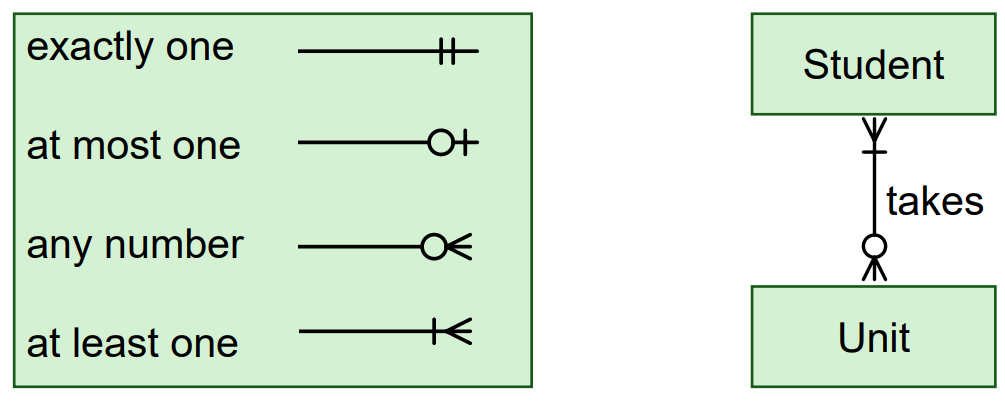
\includegraphics[width = 7cm]{crowsfoot.PNG}
\end{center} The example on the right describing the fact that a
unit is taken by at least one student and each student takes
any number of units.
\\[\baselineskip]
We can introduce intermediary entities that describe relationships
between entities. \begin{center}
    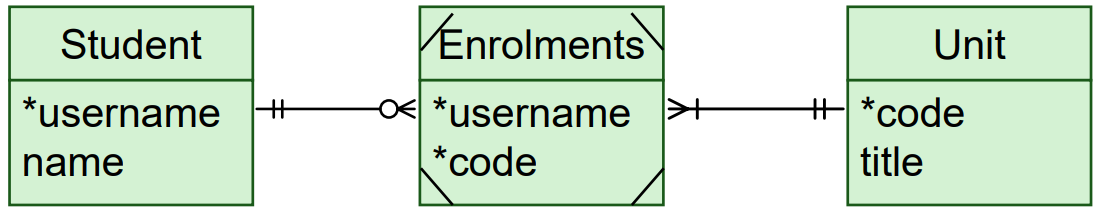
\includegraphics[width = 9cm]{associative.PNG}
\end{center} Note how the new entity is unique to the 
pair of entities it describes the relationship between.

\subsubsection{Forming Tables from Relationships}

Entities become tables, attributes become columns, entity instances
become rows. 
\\[\baselineskip]
For unique relationships between entities, we
can use a \texttt{UNIQUE} foreign key relating them. 
If two entities require each other, we merge their tables. 
Otherwise, wherever the relationship is mandatory, we place the key
(with the property \texttt{NOT NULL}) or if it isn't mandatory at all,
we can use the property \texttt{NULL}.
\\[\baselineskip]
For one-to-many relationships, we place the foreign key on the
'many' side of the relationship.
\\[\baselineskip]
For many-to-many relationships, we create a new table (a 'join' table)
containing two foreign keys to the original tables (with its 
primary key being the composite of these two foreign keys).
This table contains pairs of IDs from the original tables to 
describe relationships.

\subsection{Projection and Selection}

Projection is about selecting columns from tables whereas 
Selection is about selecting rows from tables. While
projecting, we can perform operations on our columns where
it makes sense (concatenating first and last names, adding
one, etc.). While selecting, we can provide constraints on
what records are selected.
